\section{Program Synthesis Algorithm}

\begin{figure}[t]
\centering
\includesvg[width=0.7\columnwidth]{graph.svg}
\caption{Example of a graph encoding of a state. Variables are shown in gray and objects are shown in purple. Binary relationships are shown in red (for a vertex $\rho$) and pink (for a vertex $(i,\rho_i)$). Unary relationships are shown in yellow; these relationships only have a single object, so we do not need a separate vertex for each relationship in $(i,\rho_i)$. The target relationship is shown in blue.}
\label{fig:graph}
\end{figure}

\begin{figure*}[t]
\centering
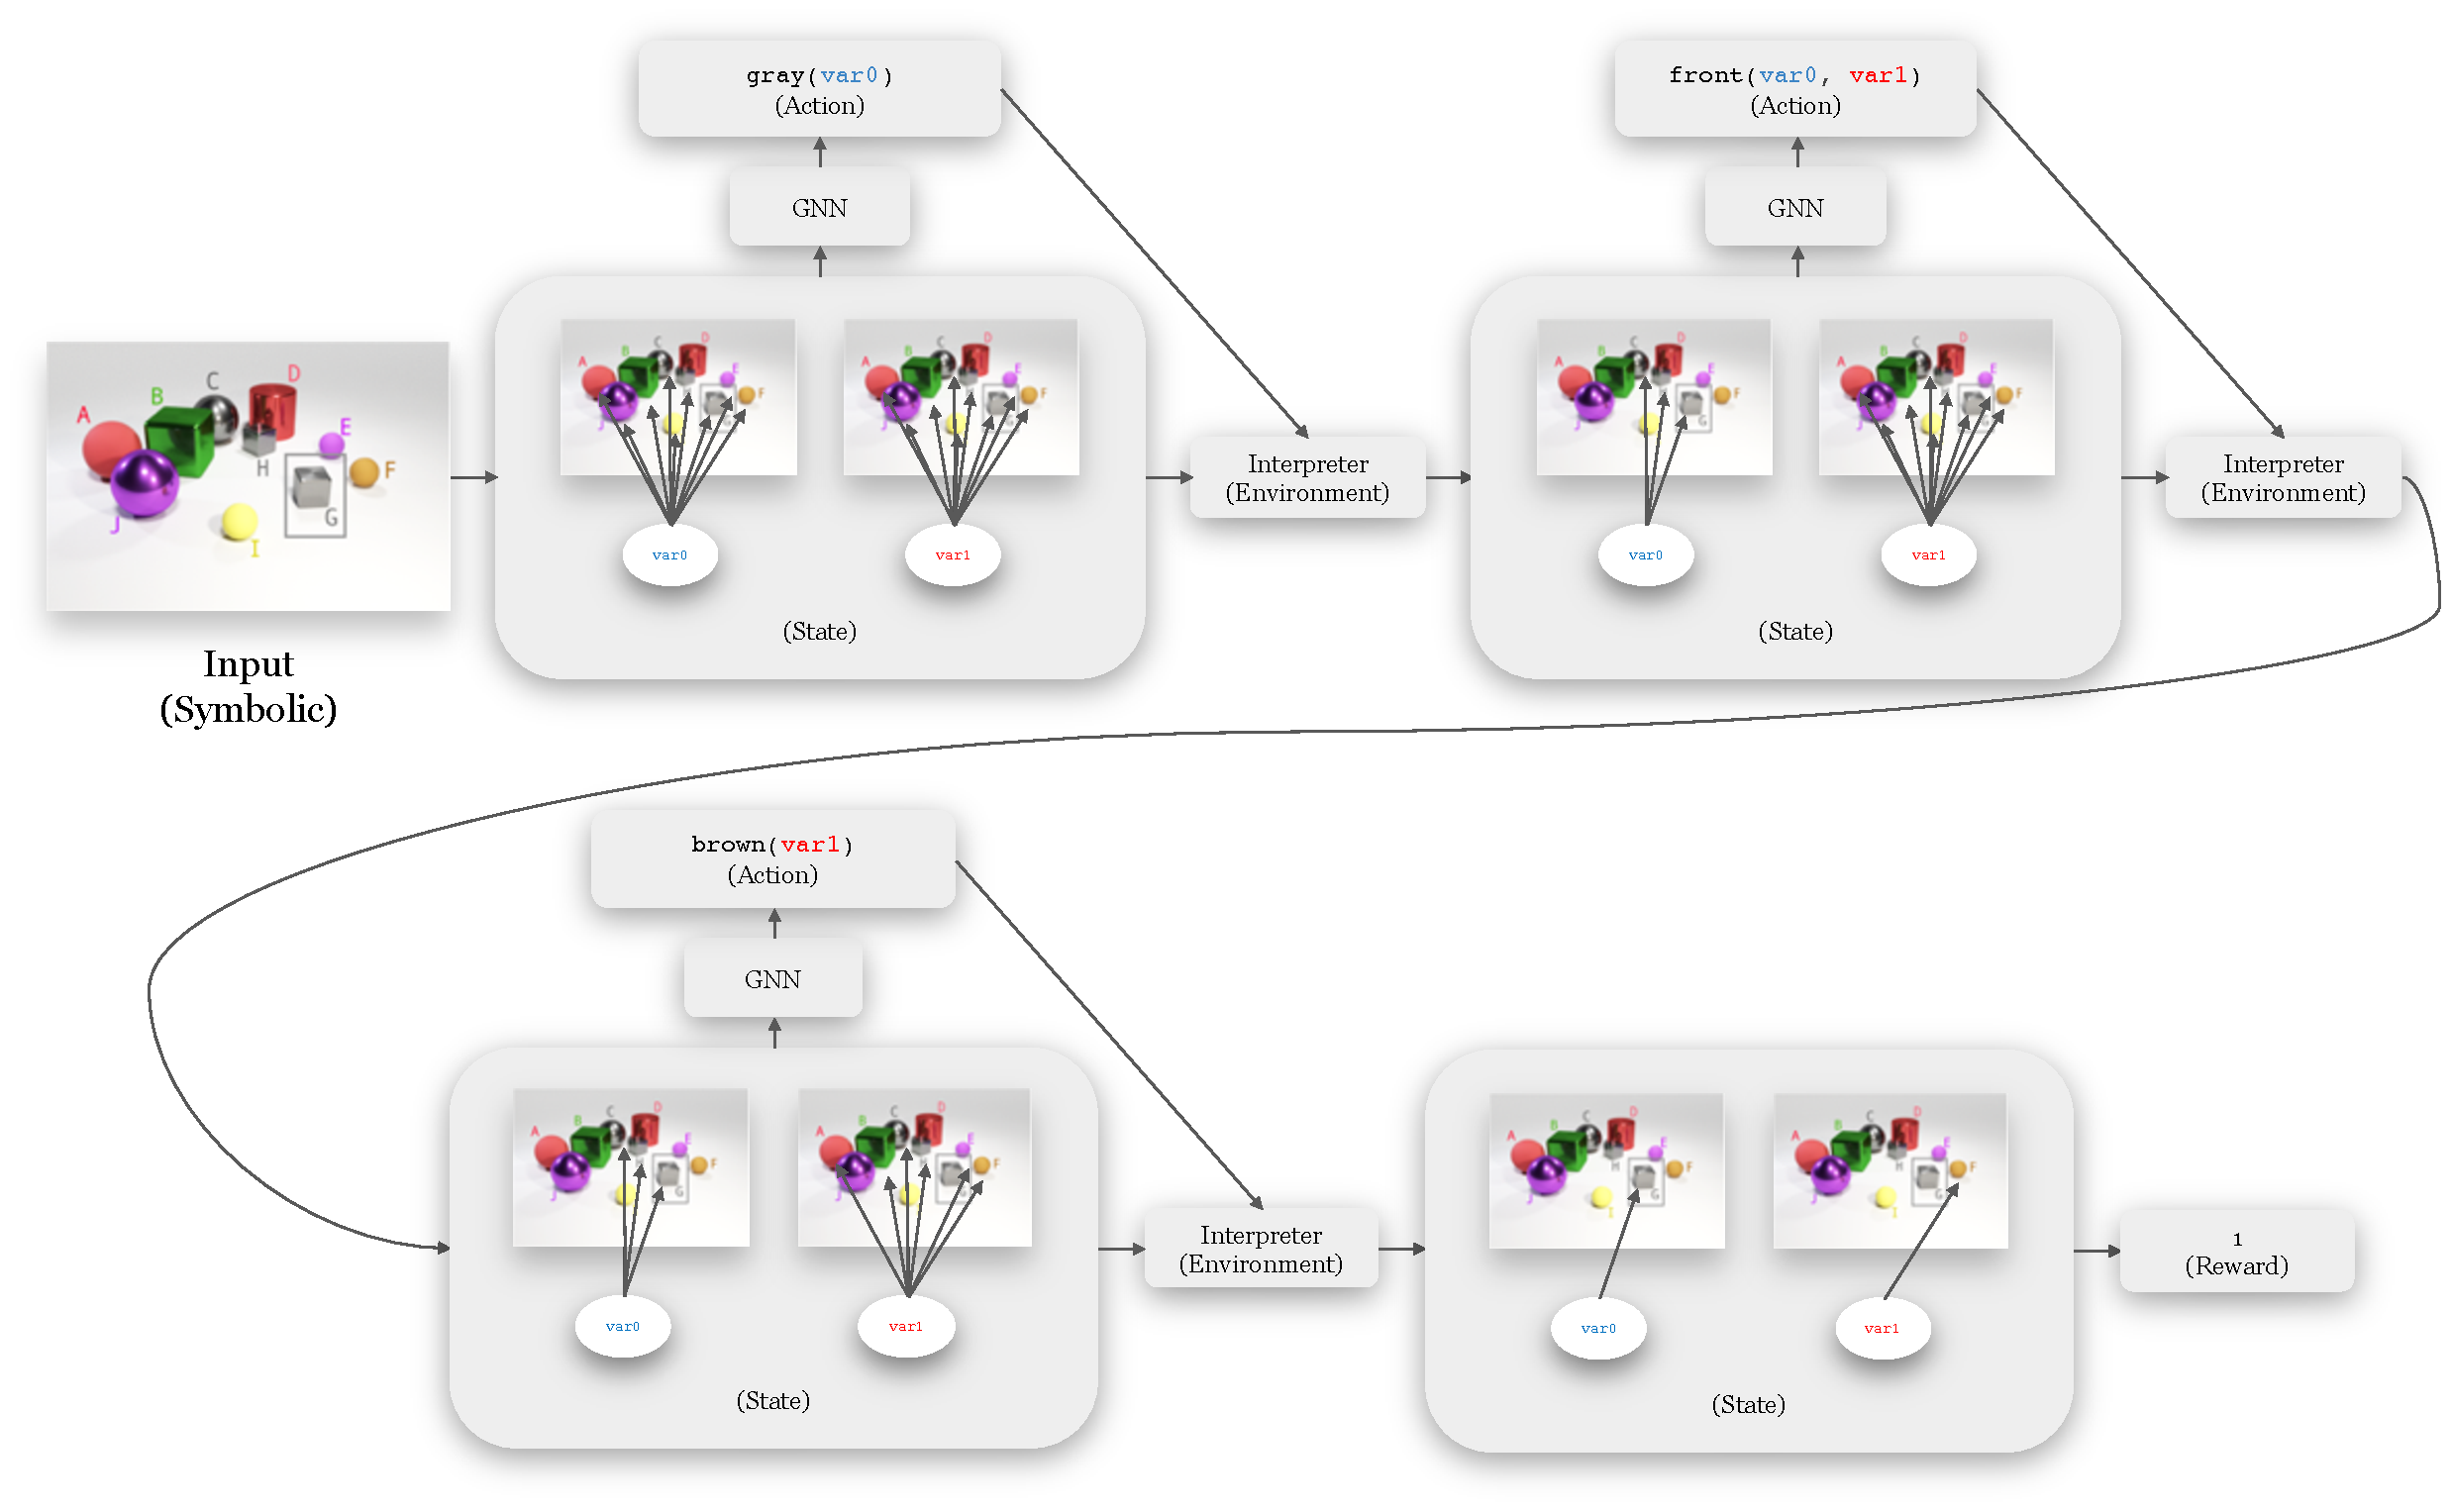
\includegraphics[width=\textwidth]{overview.pdf}
\caption{Example rollout according to our MDP. The input is a symbolic representation of the image as a graph. The states encode possible assignments of variables to objects in the scene; these are represented as graphs such as the one shown in Figure~\ref{fig:graph}. The actions are clauses $\rho(z_1,...,z_n)$; an action is chosen according to the $Q$-values predicted by the GNN $Q$-network. The interpreter, which serves as the ``environment'', removes the variables assignments that are no longer permitted by the newly chosen clause.}
\label{fig:mdp}
\end{figure*}

Next, we describe our algorithm that, given a scene graph $G$, synthesizes a referring relational program $P$ for $G$. At a high level, we formulate the synthesis problem as a Markov decision process (MDP). We then use reinforcement learning to learn a good policy $\pi$ for this MDP on a training benchmark. Then, given a new test graph $G$, we continue to fine-tune $\pi$ holding $G$ fixed, and return once we find a referring relational program $P$ for $G$. Our algorithm is summarized in Algorithm~\ref{alg:synth}.

\textbf{Formulation as an MDP.}
%
We begin by describing how to formulate the problem of synthesizing a referring relational program as a Markov decision process (MDP); Figure~\ref{fig:mdp} visualizes our MDP. Intuitively, since we want the MDP to encode a search over relational programs, one approach would be to choose the states to be relational programs $P$ and the actions to be predicates $\rho(z_1,...,z_n)$; then, taking such an action in state $P$ transitions the system to
\begin{align*}
P'=P\wedge\rho(z_1,...,z_n)
\end{align*}
While this approach is possible, the states are not very informative since they do not encode any information about the semantics of relational programs. Intuitively, a policy for this MDP would have to internally construct an interpreter for relational programs to achieve good performance.

Instead, we build on an approach known as \emph{execution-guided synthesis}~\cite{chen2018execution}, where the states are the outputs produced by executing programs $P$. Intuitively, our goal is to compute a program $P$ such that all consistent valuations uniquely identify the target object---i.e., $v(\tvar)=\tobj$. Thus, given a graph $G \in \graphs$ for the current image (which is fixed for a rollout),
we consider the output of $P$ to be the set of valuations $v \in \valuations$ that are consistent with $G$.

In particular, the states $s\in S$ in our MDP are $s=(G,V)$, where $G$ is a scene graph and $V \subseteq \valuations$ is a subset of valuations. Given a graph $G$, the initial state is $s_0=(G,\valuations)$; this choice corresponds to the empty program $P_0=\text{true}$ (so $\interp{P_0}_G = \valuations$). Next, the actions $a\in A$ in our MDP are $a=(\rho,z_1,...,z_n)\in\mathcal{R}\times\mathcal{Z}^*$,%
\footnote{Here, $*$ denotes the Kleene star---i.e., a list of variables with variable but finite length.} where $\rho$ is an $n$-ary relationship. Then, the (deterministic) transitions are
\begin{align*}
(G,V')&=T((G,V),(\rho,z_1,...,z_n)) \\
V'&=\{v\in V\mid\llbracket\rho(z_1,...,z_n)\rrbracket_v(G)\}.
\end{align*}
That is, $V'$ is the set of all valuations that are consistent with $G$ given the additional predicate $\rho(z_1,...,z_n)$. Finally, we use a sparse reward function
\begin{align*}
R((G,V))=
\begin{cases}
1&\text{if}~\forall v \in V .\ v(\tvar) = \tobj \\
0&\text{otherwise}.
\end{cases}
\end{align*}
In particular, suppose we take a sequence of actions
\begin{align*}
(\rho_1,z^1_1,...,z^1_{n_1}),...,(\rho_m,z^m_1,...,z^m_{n_m}).
\end{align*}
Then, letting $P$ be the relational program
\begin{align*}
P=\bigwedge_{i=1}^m\rho_i(z^i_1,...,z^i_{n_m}),
\end{align*}
the state $V$ after taking these actions equals is
\begin{align*}
V=\{v\in\mathcal{V}\mid\llbracket P\rrbracket_v(G)\}=\llbracket P\rrbracket_G.
\end{align*}
Thus, $R((G,V))=1$ if and only if the program $P$ corresponding to the sequence of actions taken is a referring relational program for $G$. Thus, a policy that achieves good reward on this MDP should quickly identify a valid referring relational program for a given graph $G$.

To handle uncertain relationships, we keep track of both certain and uncertain relationships---i.e., the initial state is $s_0=(G,\mathcal{V},\varnothing)$, and the transitions are
\begin{align*}
(G,V_+',V_?')=T((G,V),(\rho,z_1,...,z_n))
\end{align*}
where
\begin{align*}
V_+' =& \set{v \in V_+ \mid \interp{\rho(z_1,...,z_n)}_v(G_+)} \\
V_?' =& \set{v \in V_? \mid \interp{\rho(z_1,...,z_n)}_v(G)} \\
     &\hspace{0.1in}\cup \set{v \in V_+ \mid \interp{\rho(z_1,...,z_n)}_v(G_?)}.
\end{align*}
Finally, the rewards are as before---i.e.,
\begin{align*}
R((G,V_+,V_?))=
\begin{cases}
1&\text{if}~\forall v \in V_+ \cup V_? .\ v(\tvar) = \tobj \\
0&\text{otherwise}.
\end{cases}
\end{align*}

\textbf{Reinforcement learning.}
%
We use the deep $Q$-learning algorithm with a replay buffer to perform reinforcement learning---surprisingly, we found this approach outperformed policy gradient and actor-critic approaches. Intuitively, we believe it works well since the states in our formulation capture a lot of information about the progress of the policy. Given the deep $Q$-network $Q_{\theta}(s,a)$, the corresponding policy $\pi$ is to use $Q_{\theta}(s,a)$ with $\epsilon$-greedy exploration---i.e., $\pi(s)=\operatorname*{\arg\max}_{a\in A}Q_{\theta}(s,a)$ with probability $1-\epsilon$, and $\pi(s)\sim\text{Uniform}(A)$ with probability $\epsilon$.

\begin{figure*}[t]
\centering
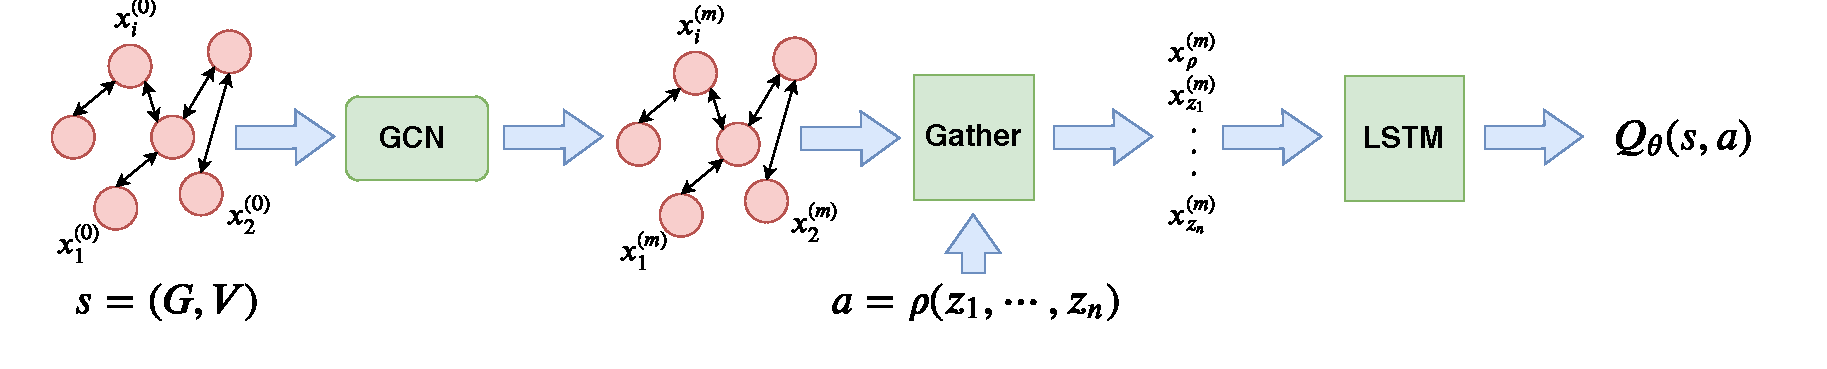
\includegraphics[width=0.95\textwidth]{Qnetwork.pdf}
\vspace{-10pt}
\caption{Our $Q$-network architecture. It takes as input an encoding of the state as a graph, and produces a vector embedding for each node using a GCN. Then, it predicts $Q(s,a)$ based on the vector embeddings for the nodes in the graph relevant to the action $a$.} 
\label{fig:mdp}
\end{figure*}

\textbf{State encoding.}
%
A key challenge is designing a neural network architecture for predicting $Q_{\theta}(s,a)$. Our approach is based on encoding $s=(G,V)$ as a graph data structure, and then choosing $Q_{\theta}(s,a)$ to be a graph neural network (GNN). Our graph encoding of $(G,V)$ has three main kinds of vertices: (i) objects $o$ in $G$, (ii) relationships $\rho\in\mathcal{R}$, and (iii) variables $z\in\mathcal{Z}$, as well as a few auxiliary kinds of vertices to support the graph encoding. In Figure~\ref{fig:graph}, we show an example of a graph encoding of a state in our MDP.

First, each object $o$ is represented by exactly one vertex in the graph; each relationship $\rho\in\mathcal{R}$ is represented by exactly one vertex in the graph; and each variable $z\in\mathcal{Z}$ is represented by exactly one vertex in the graph.

Second, for each relationship $\rho_i(o_{i,1},...,o_{i,n_i})\in G$, we introduce $n+1$ new vertices $\{(i,\rho_i),(i,1),...,(i,n_i)\}$ into the graph, along with the edges
\begin{align*}
(i,\rho_i)\to(i,1)\to o_1,...,(i,\rho_i)\to(i,n_i)\to o_{n_i}
\end{align*}
as well as the edge $\rho_i\to(i,\rho_i)$. This approach serves two purposes. The first purpose is that the intermediate vertex $(i,\rho_i)$ distinguishes different relationships in $G$ with the same type $\rho_i\in\mathcal{R}$. In addition, the edges $\rho_i\to(i,\rho_i)$ connects all relationship of the same type, which allows information to flow between these parts of the graph---for example, these edges could help the GNN count how many occurrences of the relationship ``red'' are in $G$. The second purpose is that the intermediate vertices $(i,j)$ preserve information about the ordering of the objects in the relationship---e.g., in $\text{front}(o,o')$, the edge $(i,0)\to o$ indicates that $o$ is in front, and $(i,1)\to o'$ indicates that $o'$ is behind.

Third, to encode the valuations $v\in V$, we include the following edges in the graph:
\begin{align*}
\bigcup_{v\in V}\{z\to v(z)\mid z\in\mathcal{Z}\}.
\end{align*}
Intuitively, these edges capture all possible assignments of objects $o$ to variables $z$ that are allowed by $V$. For instance, in the initial state $S_0=(G,\mathcal{V})$, these edges are $z\to o$ for every $z\in\mathcal{Z}$ and $o$ in $G$. This encoding loses information about $V$, since an assignment $o$ to $z$ may only be allowed for a subset of $v\in V$. However, $V$ is combinatorial in size, so encoding the entire structure of $V$ yields too large a graph.

To ensure that information can flow both ways, all edges in our encoding described above are bidirectional.

Finally, for settings $G=(G_+,G_?)$ where we consider uncertain relationships, we encode whether the relationship is certain as an edge type $\rho\xrightarrow{+}(i,\rho_i)$ for certain relationships in $G_+$ and $\rho\xrightarrow{?}(i,\rho_i)$ for uncertain relationships in $G_?$. Similarly, we use $z\xrightarrow{+}v(z)$ for certain valuations $v\in V_+$ and $z\xrightarrow{?}v(z)$ for uncertain valuations $v\in V_?$.

\textbf{Neural network architecture.}
%
As mentioned above, $Q_{\theta}(s,a)$ is based on a graph convolutional network (GCN)~\cite{kipf2016semi}. We use $\psi(s)$ to denote the graph encoding of $s=(G,V)$ described above, where in addition each node is represented by a fixed embedding vector depending on its node name. The relationship vertices $\rho$ and $(i,\rho_i)$ have an embedding vector $x_{\rho}$. The positional vertices $(i,j)$ encoding object ordering use an single embedding $x_{\rho_i,j}$ specific to both the corresponding relationship $\rho_i$ and the object position $j$ within the relationship.

Now, $Q_{\theta}$ applies a sequence of graph convolutions to $\psi(s)$:
\begin{align*}
\psi^{(0)}&=\psi(s) \\
\psi^{(t+1)}&=f_{\theta}^{(t)}(\psi^{(t)})\hspace{0.1in}(\forall t\in\{0,1,...,m-1\}.
\end{align*}
Each $\psi^{(t)}$ has the same graph structure as $\psi(s)$, but the embedding vectors $x_k^{(t)}$ associated with each vertex $k$ are different (i.e., computed as a function of the embeddings in the previous layer and of the GCN parameters).

Finally, at the output layer, $Q_{\theta}$ decodes the $Q$-values for each action $\rho(z_1,...,z_n)$ based on the embedding vectors of the corresponding vertices $\rho,z_1,...,z_n$:
\begin{align*}
Q_{\theta}(s,\rho(z_1,...,z_n))=g_{\theta}(x_{\rho}^{(m)},x_{z_1}^{(m)},...,x_{z_n}^{(m)})
\end{align*}
The architecture of $g_{\theta}$ can be any aggregation method from vertex level to action level. Two example strategies are LSTM structure and concatenation. 

\textbf{Hierarchical synthesis.}
%
We adopt an approach based on \emph{hierarchical synthesis}~\cite{nye2019learning}. The idea is to combine a neurosymbolic synthesizer with a traditional one based on enumerative search. Intuitively, the neurosymbolic synthesizer can determine the majority of the program, after which the enumerative synthesizer can be used to complete the program into one that satisfies $\phi_G(P)$.

More precisely, in the first phase, we run the neurosymbolic synthesizer for a fixed number $N$ of steps. At each step in this phase, we generate a program $P$ of length $M$; if we find one that satisfies $\phi_G(P)$, then we return it. Otherwise, we continue to the second phase. In this phase, we begin by constructing the best program $P^0$ of length $M-K$ according to $Q_{\theta}$ (i.e., use zero exploration $\epsilon=0$), where $K\in\mathbb{N}$ is a hyperparameter of our algorithm. Then, we perform an exhaustive search over programs $P$ of length $K$, checking if the combined program $P'=P^0\wedge P$ satisfies $\phi_G(P')$. If we find such a program, then we return it. Finally, we return $\varnothing$ if we do not find a valid program, indicating failure.  

\textbf{Meta-learning.}
%
Finally, the algorithm we have described so far is for synthesizing a single referring relational program from scratch for a given scene graph $G$. We use a simple meta-learning approach where we pretrain $Q_{\theta}$ on a training benchmark of similar synthesis problems. In particular, we assume given a training set $\mathcal{G}_{\text{train}}\subseteq\mathcal{G}$ of scene graphs; then, we use deep $Q$-learning to train a neural network $Q_{\theta^0}$ that achieves high reward on average for random 
\begin{align*}
\theta^0=\operatorname*{\arg\max}_{\theta}\mathop{\mathbb{E}}_{G\sim\text{Uniform}(\mathcal{G}_{\text{train}})} \;[J(\theta;G)],
\end{align*}
where $J(\theta;G)$ is the standard $Q$-learning objective for the MDP constructed for scene graph $G$.

\textbf{Overall algorithm.}
%
Our overall algorithm is summarized in Algorithm~\ref{alg:synth}. It takes as input a scene graph $G$, and outputs a relational referring program $P$ (i.e., that satisfies $\phi_G(P)$), or $\varnothing$ if it fails to find such a program. The first step initializes $Q_{\theta}$ with the pretrained parameters $\theta^0$. Then, the first phase uses deep $Q$-learning to tune $\theta$ based on programs $P$ of length $M$ sampled from the MDP for $G$. If no valid program is found, then it proceeds to the second phase, where it performs an exhaustive enumerative search over programs $P^0\wedge P$, where $P^0$ is the optimal program of length $M-K$ according to $Q_{\theta}$. If again no valid program is found, then it returns $\varnothing$ to indicate failure.